\newpage


\section{Experimento 2}

\subsection{Sensores que utiliza}

Los sensores que utiliza la máquina son los mostrados en las imágenes a continuación, y corresponden a bancos de prueba de un motor.
 
La primera imagen corresponde a una celda de carga o sensor de torque que es un transductor de fuerza el cual va conectado al brazo del freno del motor, para medir la fuerza de torsión que el motor está ejerciendo.\\

La segunda y tercera imagen corresponde a un sensor de velocidad, un sensor magnético o inductivo.\\

La ultima imagen corresponde a la carcasa metálica que corresponde al cuerpo del freno dinamométrico o del motor del banco de prueba.



\subsection{Imagenes}

\begin{figure}[H]
	\centering
	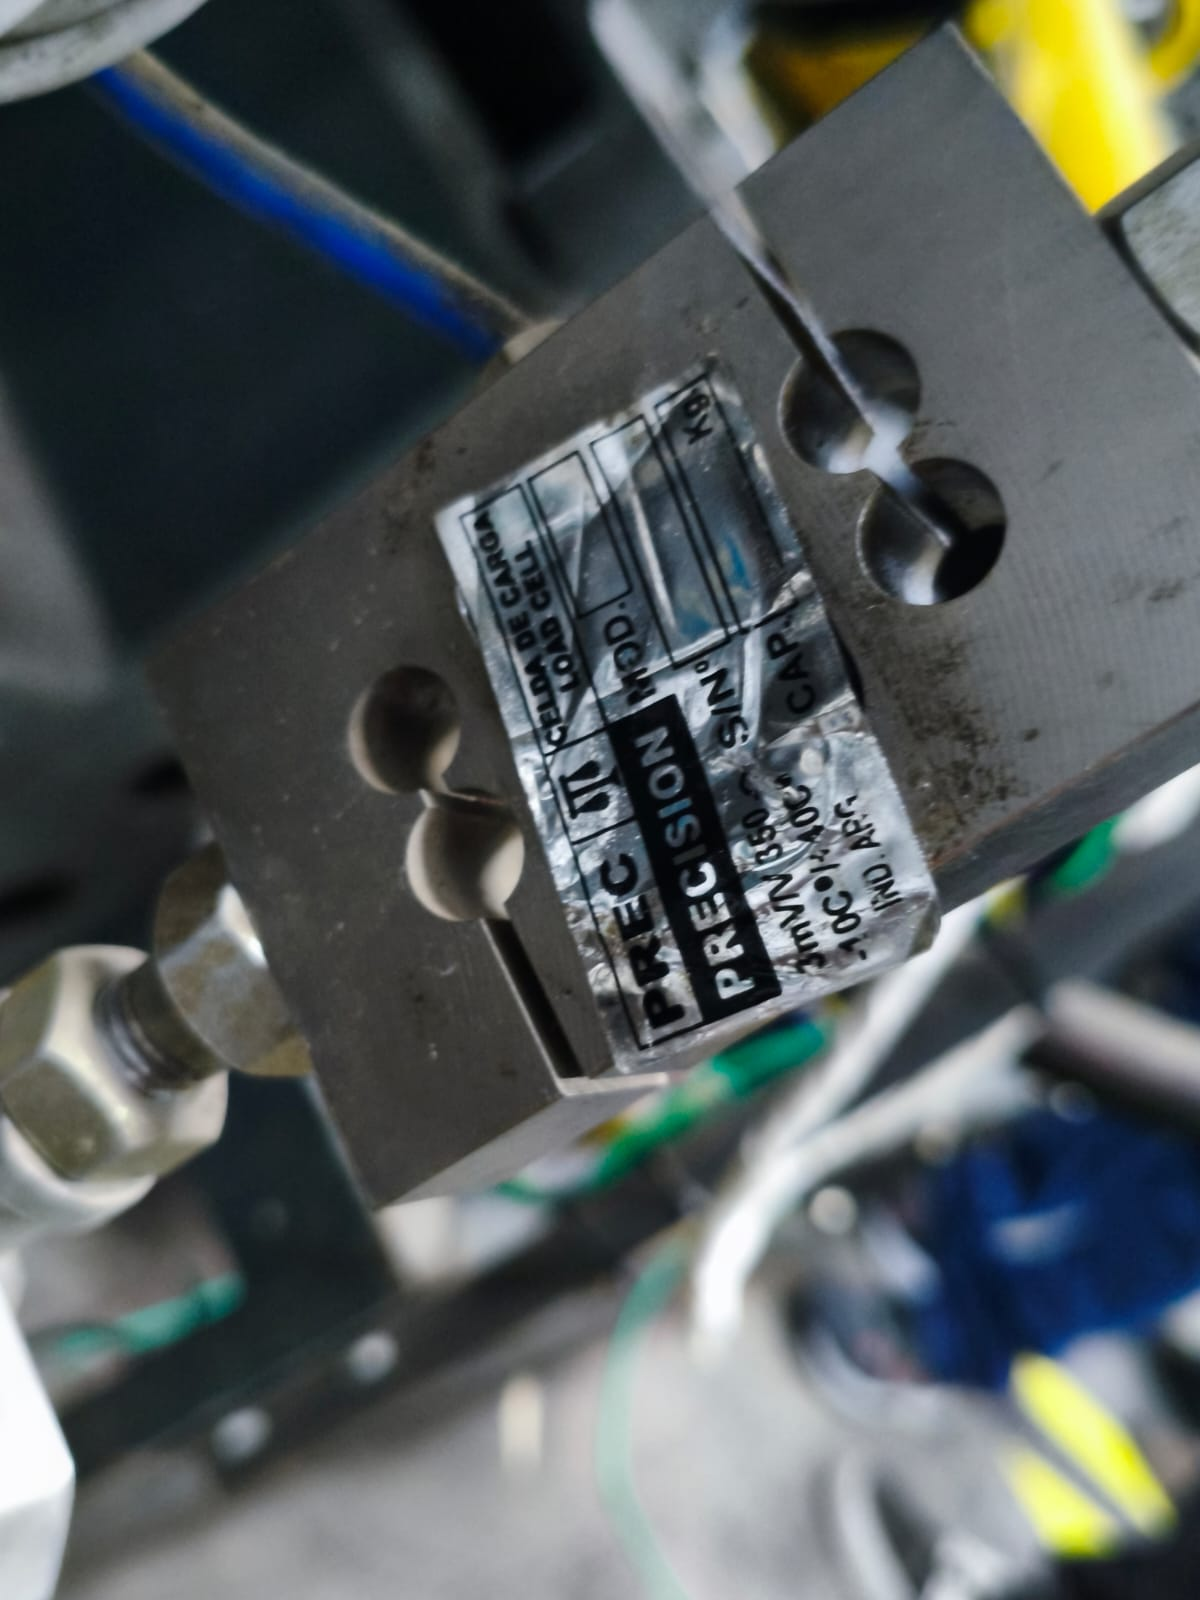
\includegraphics[width=0.7\columnwidth]{images/motor1}
	\caption{Celda de carga o sensor de torque.}
\end{figure}

\begin{figure}[H]
	\centering
	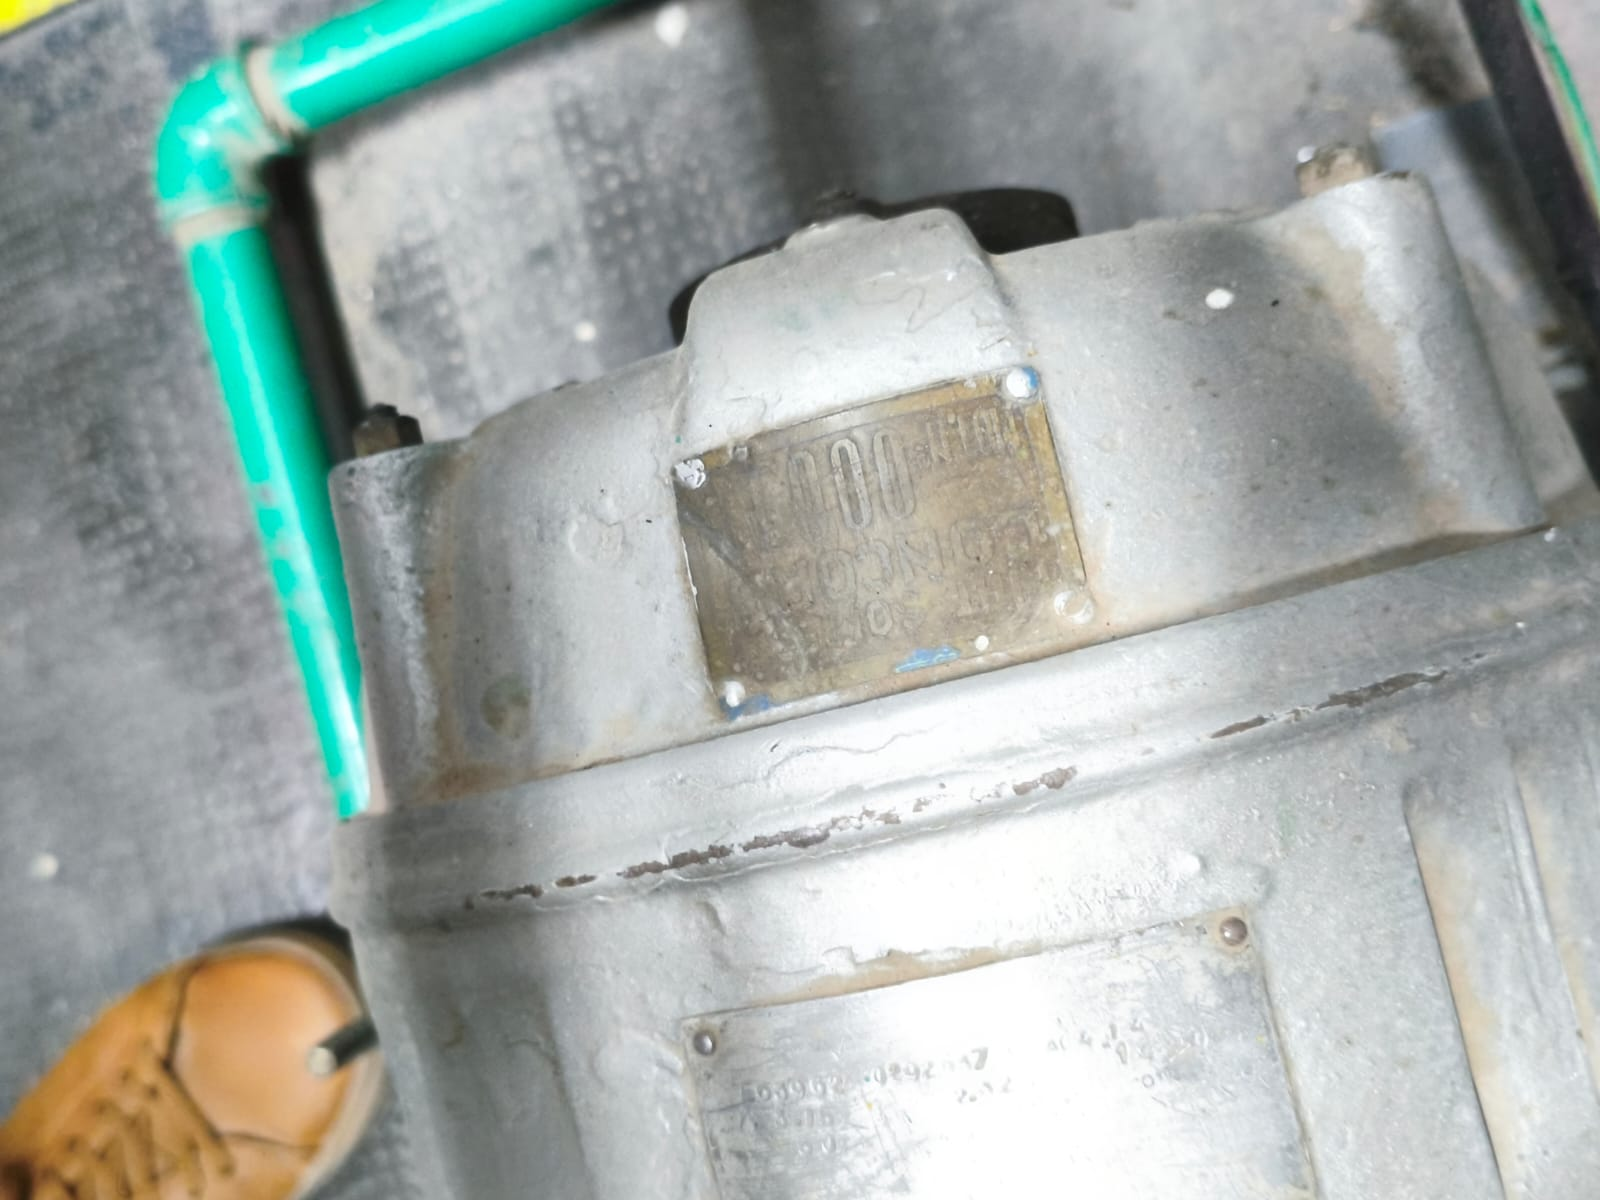
\includegraphics[width=0.8\columnwidth]{images/motor4}
	\caption{Carcasa metálica del freno dinamométrico o motor.}
\end{figure}

\begin{figure}[H]
	\centering
	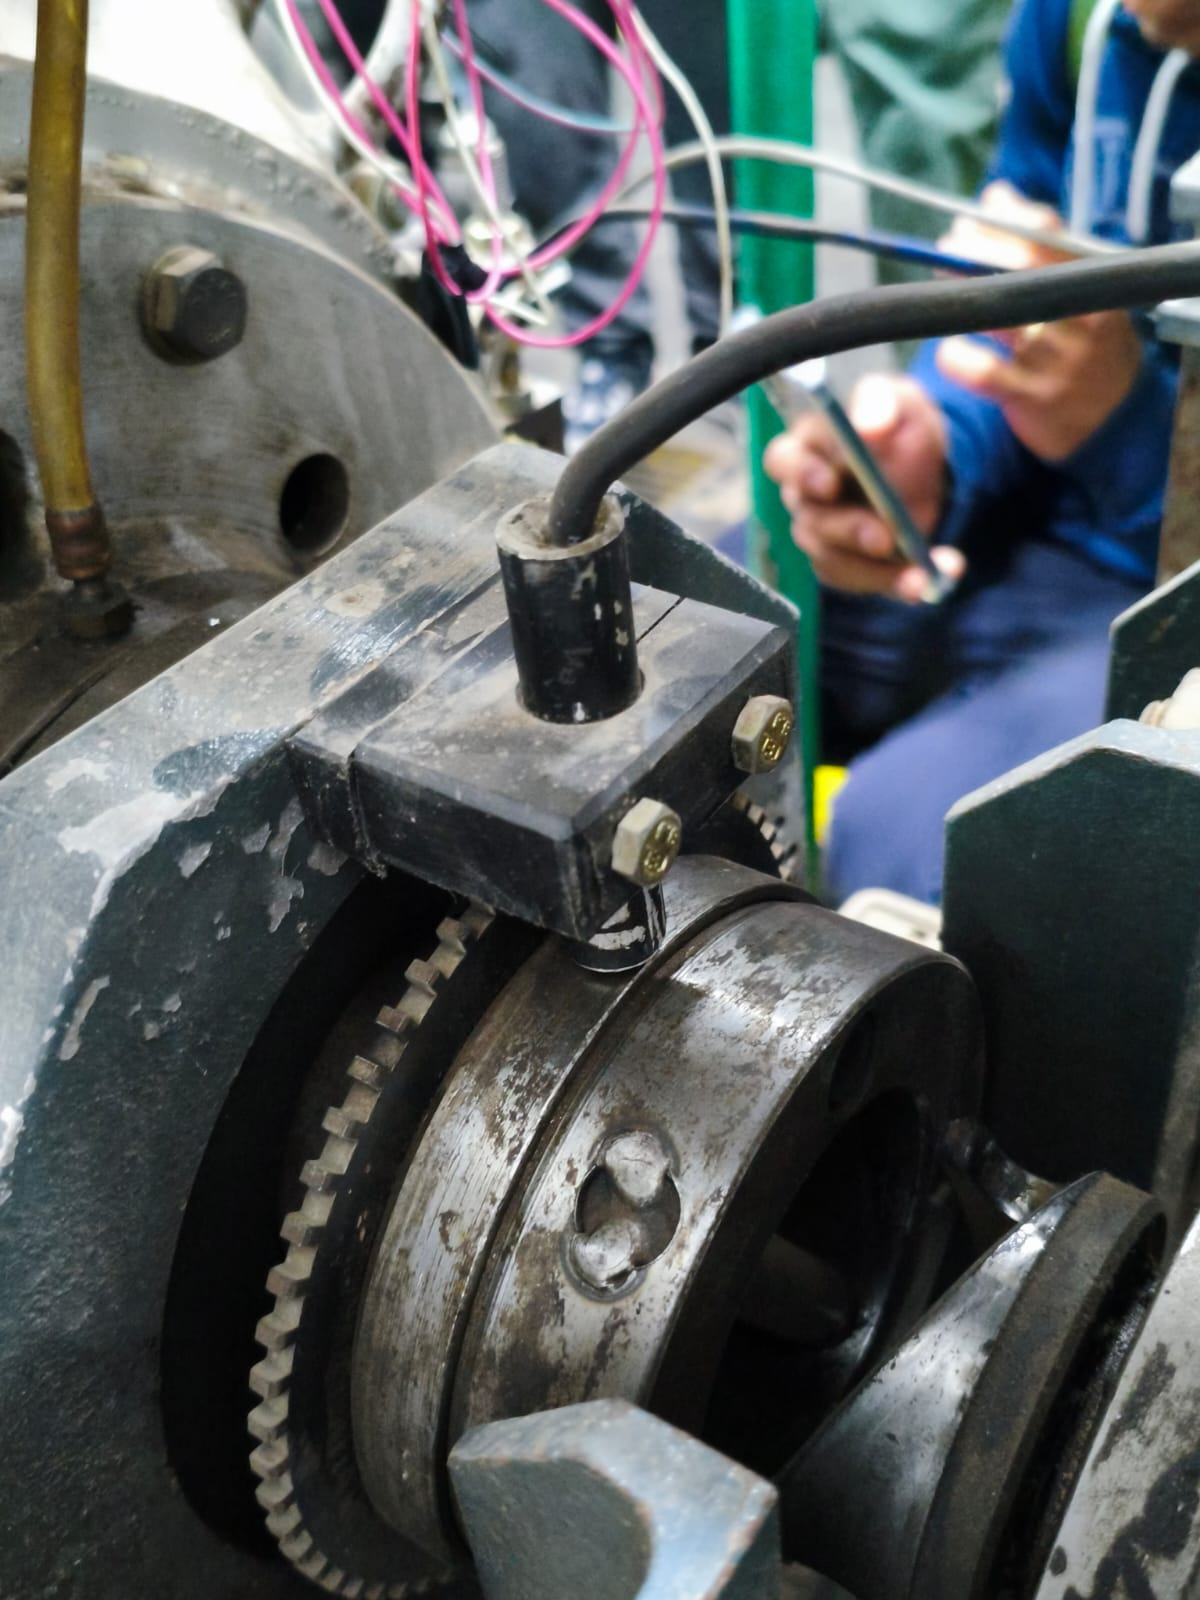
\includegraphics[width=0.8\columnwidth]{images/motor2}
	\caption{Sensor de velocidad magnético o inductivo.}
\end{figure}

\begin{figure}[H]
	\centering
	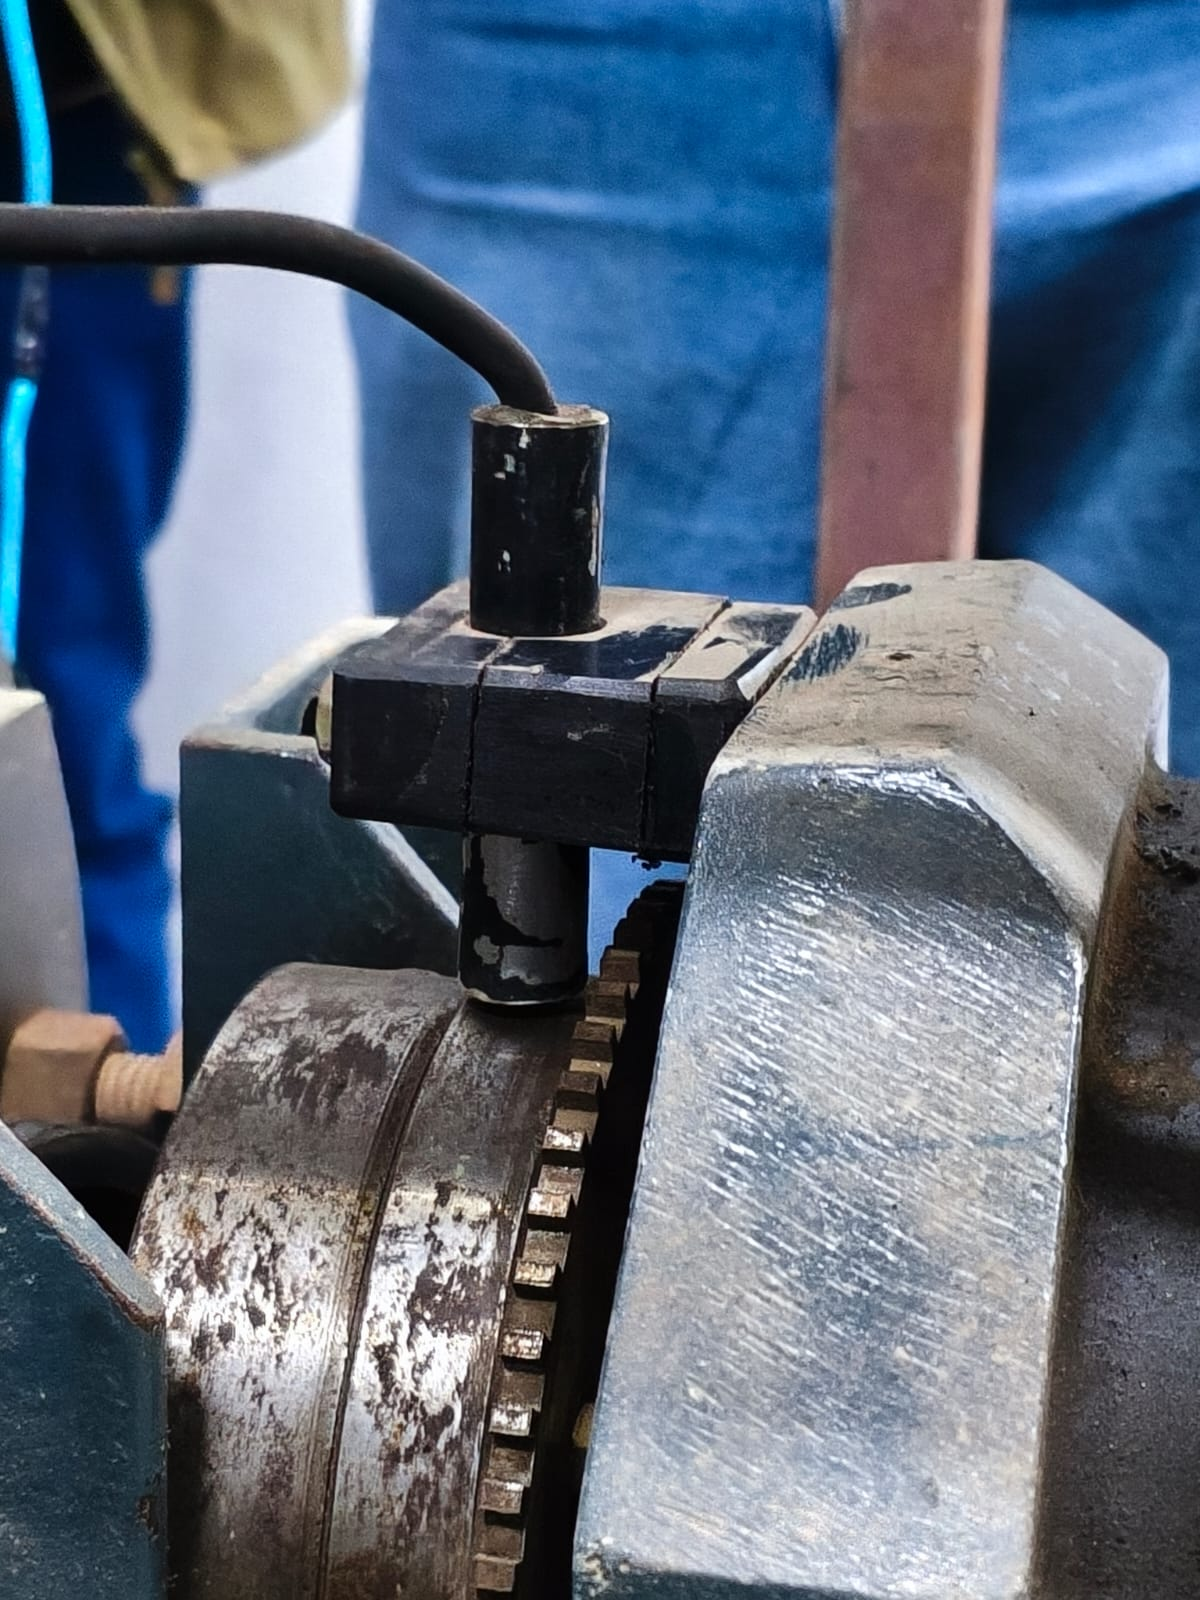
\includegraphics[width=0.8\columnwidth]{images/motor3}
	\caption{Sensor de velocidad magnético o inductivo.}
\end{figure}





